%\documentclass[10pt,preprint]{aastex}
\documentclass[apj]{emulateapj}
\usepackage{txfonts}
\usepackage{graphicx}
\usepackage{natbib}

\newcommand{\kms}{${\rm km \; s^{-1}}$}

\shorttitle{Local Number Density Environments of Massive Galaxies}
\shortauthors{Lifset}

\begin{document} 
\title{Local Number Density Environments of Massive Galaxies}

\author{Noah Lifset\altaffilmark{1}, 3D-HST}
\altaffiltext{1}{Yale University, 260 Whitney Ave., New Haven, CT 06511}

\begin{abstract}

We study the local galaxy number density environments of very massive galaxies in the 3d-hst survey. We select galaxies with mass greater than 10 \textsuperscript{11} solar masses and with a redshift between 0.5 and 2.5. Using both the nth nearest and counts in aperture radius calculations for galaxy number density, we are able to study both the immediate environment and general environment. Sorting the galaxies into  redshift and mass bins, we study the relationship between local galaxy number density, redshift, and mass. We also look at galaxy conformity through the number density of star-forming satellites compared to star-forming central galaxies. A FEW SENTENCES ABOUT RESULTS.
\end{abstract}
\keywords{}

\section{Introduction}

The properties of galaxies are largely affected by their local environments and vice-versa. Local galaxy environments have been shown to correlate with a number of important properties, such as morphology, mass, star formation rate, and stellar colors. Less is known, though, about local galaxy environment and redshift, especially at  $z$\textgreater1. One of the most powerful tools for studying local galaxy environment is looking at the local galaxy number density for a selected sample of galaxies. Binning the central or satellite galaxies based on certain properties can allow a serious analysis of the prevalence of various galaxy properties in the local environments of selected central galaxies. 

In this paper, we use two of the most common methods for calculating galaxy number density around selected central galaxies: counts in aperture radius and nth nearest galaxy. Counts in aperture radius allow us to study galaxy number density in both the immediate local environment as well as the more general environment depending on what aperture radius is selected. The nth nearest galaxy method can be used to show both local and general environment, but it is most commonly used for just the local environment. This is because it is more accurate in depicting galaxy number density at small radii ~\cite{2005ApJ...634..833C}. 

We study a few different galaxy properties using these methods in this paper. We look at the difference in local galaxy number density dependign on both central galaxy mass and  satellite galaxy mass. We also look at evolution in galaxy number density with redshift of the central galaxy. Finally, we study galaxy conformity through star-forming and quiescent central and satellite galaxies. Binning the central and satellite galaxies based on these properties allows us to use our galaxy number density calculation methods to study the prevalence of these galaxy properties in the local and general environments.

For this paper we adopt the following cosmological parameters: $\Omega_{m}$ = 0.3, $\Omega_{\Lambda}$ = 0.7, and \textit{H}$_{0}$ = 69.31 km (s Mpc)$^{-1}$.

\section{Sample Selection}

We use data from the galaxy survey 3d hst, which includes the fields Aegis, Cosmos, Goods-n, Goods-s, and uds. For our sample of massive galaxies to study, we made a few specifications. Galaxies are selected with a mass greater than 10 \textsuperscript{11} solar masses, although none exceed 10 \textsuperscript{11.8}. We also limit ourselves to galaxies within a redshift range of 0.5 to 2.5. In order to avoid errors in the calculation from selecting galaxies at the edge, and thus getting a less than expected number density, we do not select galaxies within 0.05 degrees of the edges of any field used.
We must also limit the selection of general galaxies used to calculate local number density. We only use galaxies within the same redshift range and with mass greater than 10 \textsuperscript{9,415} solar masses. The lower mass limit was taken from Tal (2014)~\cite{2014ApJ...789..164T}, and is used to keep completeness above 95\% at all redshifts.

\section{Data and Analysis}

We use two different methods for calculating local galaxy number density. The first, the nth nearest neighbor calculation, has been shown to be more accurate for immediate environments Cooper (2005)~\cite{2005ApJ...634..833C}. The second, counts in selected aperture radius, is more accurate for larger and more general environments Cooper (2005)~\cite{2005ApJ...634..833C}.

\subsection{Nth Nearest Calculation}

One of the most common ways of measuring local galaxy number density is using the distance to the nth nearest spectroscopically observed galaxy. Redshift information is used to restrict the pool of neighbors that can be selected from to a given velocity interval. This is done to avoid background and foreground sources. A redshift difference of 0.08 is used here to try and maintain completeness as best as possible. This cut off was selected based on suggestions by Cooper (2005)~\cite{2005ApJ...634..833C}, Tal (2012)~\cite{2012ApJ...751L...5T}, and Muldrew (2012)~\cite{2012MNRAS.419.2670M}. Thus the pool of galaxies that the nth nearest neighbor is being selected from is a cylinder, rather than a sphere. The nth nearest neighbor distance is expressed as a projected surface density $\Sigma$ $_{n}$. The calculation for the projected surface density is

 $$\Sigma_{n} = n / (\pi  R_{n}^{2})$$

 where R$_{n}$ is the distance to the nth nearest neighbor. 

It should be noted that there is no subraction of average background number density, unlike the counts in aperture radius method.



\subsection{Counts in Aperture Radius Calculation}

Another method for measuring local galaxy number density is counting the number of galaxies within a certain aperture radius. This method once again requires a redshift cut of 0.08. This was selected based on the relative photometric uncertainty between selected massive galaxies and general galaxies near them. The pool of galaxies counted is then also a cylinder rather than a sphere. The calculation for galaxy number density is simply
 $$\Sigma_{r} = n_{gal} / (\pi r^{2})$$
 where r is the selected aperture radius and n$_{gal}$ is the number of galaxies within that radius. Selecting many different aperture radii allows us to analyze the galaxy number density in both local and general environments. The larger aperture radii selected show the average number density within that entire radius, while smaller aperture radii are able to show the usually increased number density within a smaller radius.

In order to calculate the galaxy number density that is solely a result of the selected massive galaxies, an average background number density is subtracted after each normal $\Sigma_{r}$ calculation. In order to do this, for each selected massive galaxy, four different calculations are carried out for galaxy number density using the selected galaxy's field and redshift, but random coordinateswithin said field. These four calculations are then averaged and we have our averaged background number density. Subtracting this from our normal $\Sigma_{r}$ calculation yields a fairly accurate representation of galaxy number density that is a direct result of the massive selected galaxies. The initial $\Sigma_{r}$, average background number density, and final calculated number density of our data can be seen in figure~\ref{fig:compare}.

This method is a variation of the one used in Tal (2013)~\cite{2013ApJ...769...31T}.

\begin{figure}
\figurenum{1}
\centering
\graphicspath{{C:/3d_hst/2015_finals/aperture_distance/}}
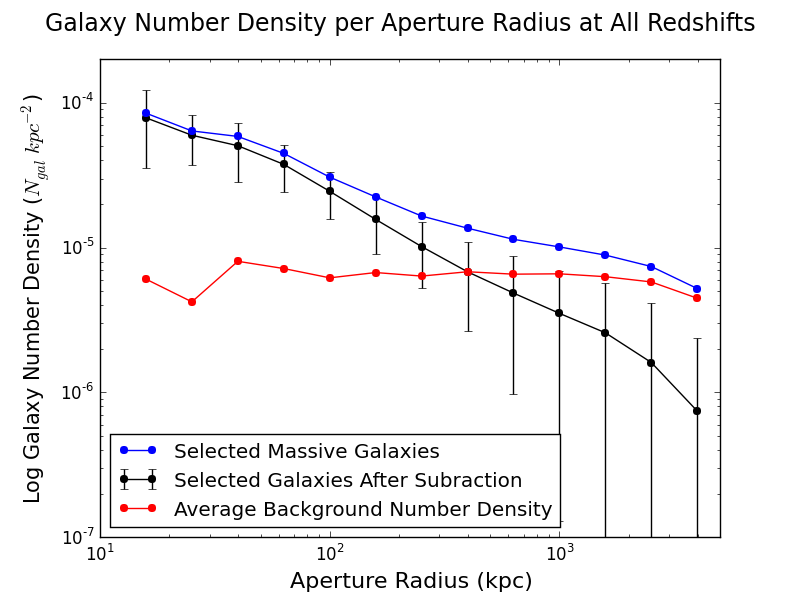
\includegraphics[width=\linewidth]{temp_compare}
\DeclareGraphicsExtensions{.png}
\caption{\footnotesize All galaxies plotted with number density compared to selected aperture radius. The average background number density per aperture radius is also included in red. The black line represents the average background number density subtracted from the calculated number density for all galaxies. The error bars show one standard deviation of thenumber density of the randomly selected background points at each aperture radius (the data used for the red line).}
\label{fig:compare}
\end{figure}

\subsection{Star-Formation Rate}

We also look at the star-formation rates of both the cenrtal and satellite galaxies. Using a rest frame U-V versus V-J graph, we sort the galaxies, central and satellite, into quiescent and star-forming groups. The vast majority of central galaxies are star-forming as can be seen in figures ~\ref{fig:color_mass} and ~\ref{fig:color_z}. There is a fairly even distribution of masses within the quiescent and star-forming groups, as well as overall. Higher redshift galaxies, however, tend to be in the upper left of the plot, indicating that they are more dusty. The potential satellite galaxies are also sorted into quiescent (3132) and star-forming (19030) groups. The overwhelming majority of star-forming satellite galaxies can be partly explained by the high mass cut-off of the central galaxies compared to the lower one of the potential satellites, which leads to a statistical domination of the sample by natural galaxy trends. 

\begin{figure}
\figurenum{2}
\centering
\graphicspath{{C:/3d_hst/2015_finals/Colors/}}
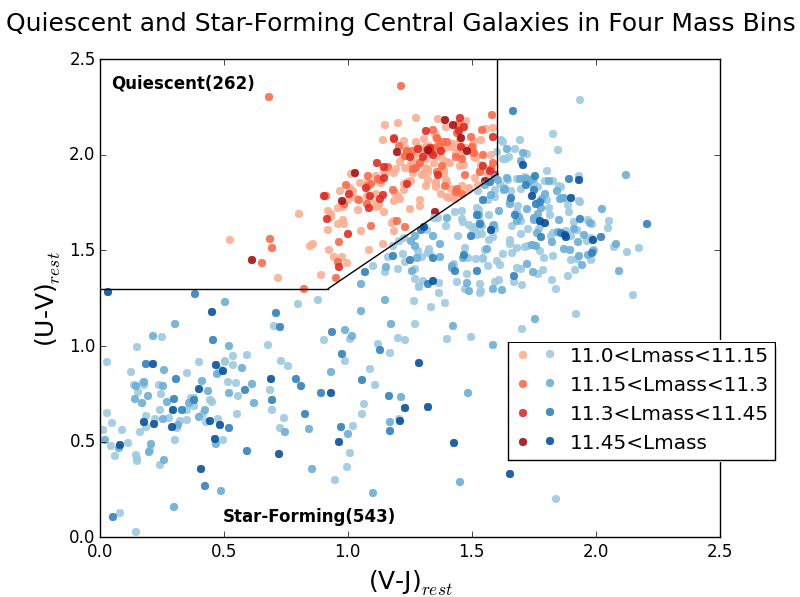
\includegraphics[width=\linewidth]{temp_color_final}
\DeclareGraphicsExtensions{.png}
\caption{\footnotesize All central galaxies on a rest frame U-V versus V-J plot. The galaxies are in four mass bins ranging from 10 \textsuperscript{11} to 10 \textsuperscript{11.8} solar masses. The vast majority of galaxies are still star-forming. There is an even distribution of masses in all areas of the plot.}
\label{fig:color_mass}
\end{figure}

\begin{figure}
\figurenum{3}
\centering
\graphicspath{{C:/3d_hst/2015_finals/Colors/}}
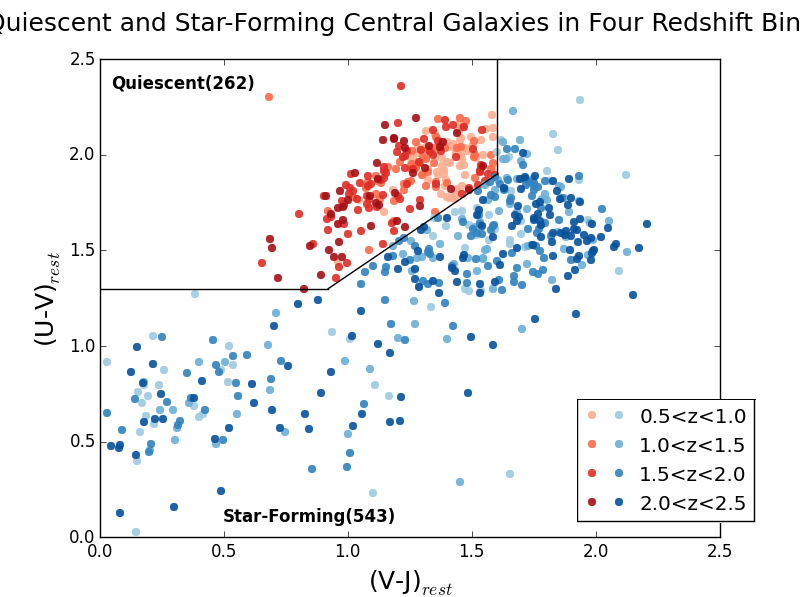
\includegraphics[width=\linewidth]{color}
\DeclareGraphicsExtensions{.png}
\caption{\footnotesize All central galaxies on a rest frame U-V versus V-J plot. The galaxies are in four redshift bins ranging from 0.5 to 2.5. The vast majority of galaxies are still star-forming. There generally higher redhsift galaxies in the upper left of the plot, indicating more dusty galaxies.}
\label{fig:color_z}
\end{figure}

\subsection{Error Estimates}

A great source of error is the variation within the random background calculations for the aperture radius method. Beyond averaging four separate calculations, we show error bars for one standard deviation of the distribution of random background calculations for each galaxy within each radius. At low aperture radii, only a handful of galaxies in our sample selection actually conatain other galaxies. As a result, the average points in this data for low aperture radii are less accurate due to being averages of only a handful of galaxies rather than a few hundred. The radii affected by this are really only the lowest three. These two sources representsthe statistical uncertainty of our calculations.

There are various systematic unccertainties that could affect our data as well. Innacuracy in redshift and mass measurements could move galaxies in and out of both the general selected sample as well as specific bins within the sample. At extremely small aperture radii, source blending could cause a smaller than expected number density. 

\section{Results}

We primarily look at the evolution of local galaxy number density with respect to change in redshift, as Tal (2013)~\cite{2013ApJ...769...31T} did, but also with respect to mass. The main method we use is is counts in aperture radius, to allow analysis of both local and general environment, but the nth nearest method was also used to provide a more accurate study of the local environment.

\subsection{Redshift Evolution}

In studying the variation in galaxy number density with respect to redshift, we split the selected massive galaxies into four bins based on redshift: 0.5 \textless  $z$ \textless 1.0, 1.0 \textless  $z$ \textless 1.5, 1.5 \textless  $z$ \textless 2.0, and 2.0 \textless  $z$ \textless 2.5. We plot these four bins on a counts in aperture radius graph to show the variation in galaxy number density over different sized environments. The smaller aperture radii are less accurate due to a lack of statistical completeness. From the third aperture radius (about 40 kpc) on, one can assume sufficient statistical completeness due to most galaxies having at least a few others within that range. In a similar manner, the last two aperture radii (about 2.5 and 4 mpc) are slightly statistically incomplete due to many galaxies containing most of their entire field within that range. We see in figure~\ref{fig:z} that there is a clear trend for the majority of the plot. Lower redshifts correspond with higher galaxy number density, and high redshifts with low densities. 

\begin{figure}
\figurenum{4}
\centering
\graphicspath{{C:/3d_hst/2015_finals/aperture_distance/}}
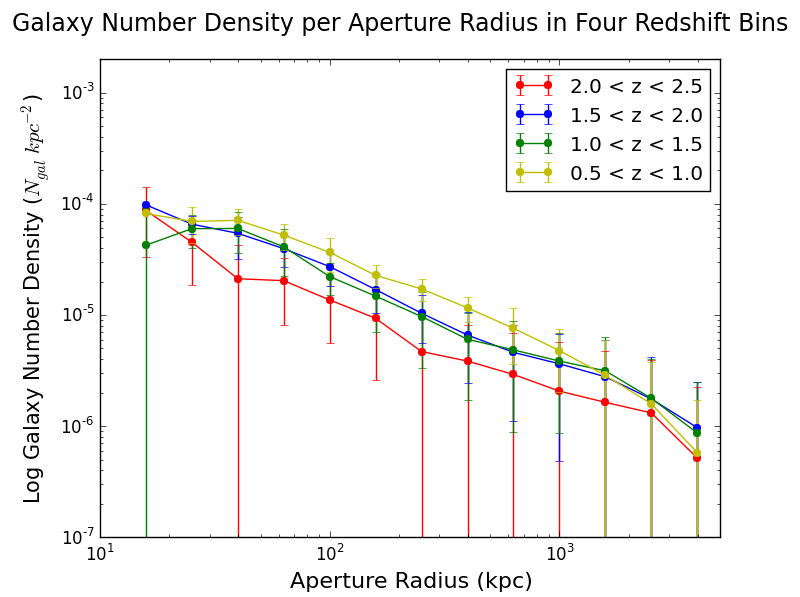
\includegraphics[width=\linewidth]{temp_z_final}
\DeclareGraphicsExtensions{.png}
\caption{\footnotesize All galaxies plotted in four redshift bins from 0.5 to 2.5. Galaxy number density is plotted with respect to aperture radius selected, both on logarithmic scales.  The lower redshifts have an increased galaxy number density in the aperture radius range of about 30 kpc to 1 mpc. Both extremes of the aperture radii can be largely ignored due to statistical incompleteness.}
\label{fig:z}
\end{figure}

We also compare this data with lower redshifts of the same plot from Tal (2013)~\cite{2013ApJ...769...31T} in figure~\ref{fig:zpanel}. Here we can see that his data shows a lower galaxy number density throughout, which can be attributed to the fact that he is using a different survey. Although the data seems very similar, Tal finds no evolution in galaxy number density with change in redshift, an interesting contrast with our data. 

\begin{figure}
\figurenum{5}
\centering
\graphicspath{{C:/3d_hst/2015_finals/aperture_distance/}}
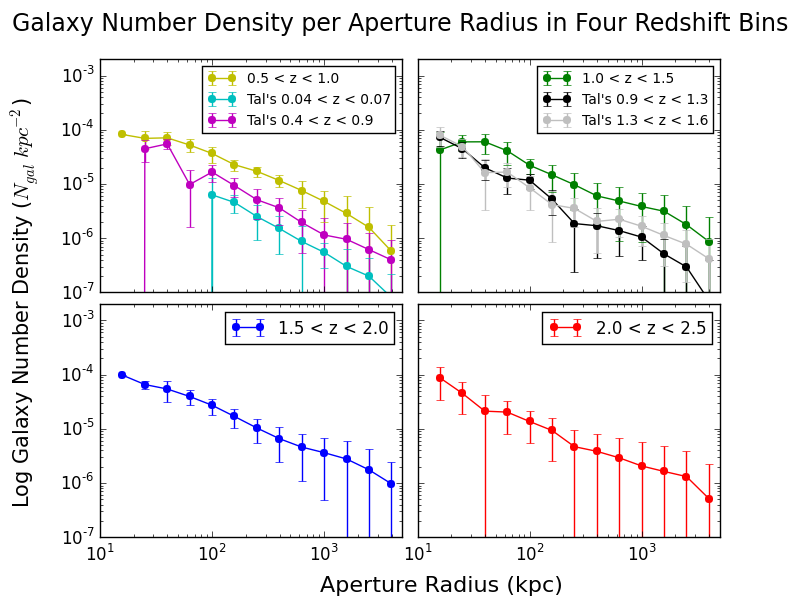
\includegraphics[width=\linewidth]{temp_zpanel_final}
\DeclareGraphicsExtensions{.png}
\caption{\footnotesize All galaxies in four mass bins plotted in a counts in aperture radius graph. Data from Tal (2013)~\cite{2013ApJ...769...31T} is also shown. Although the data is similar, Tal finds no correlation between galaxy number density and central galaxy redshift.}
\label{fig:zpanel}
\end{figure}

\subsection{Variation over Central Galaxy Mass}

In studying variation over mass, we once again split the selected massive galaxies into four mass bins: 10 \textsuperscript{11.0}$M_{\odot}$ \textless mass \textless 10 \textsuperscript{11.15}$M_{\odot}$, 10 \textsuperscript{11.15}$M_{\odot}$ \textless mass \textless 10 \textsuperscript{11.3}$M_{\odot}$, 10 \textsuperscript{11.3}$M_{\odot}$ \textless mass \textless 10 \textsuperscript{11.45}$M_{\odot}$, and mass \textgreater 10 \textsuperscript{11.45}$M_{\odot}$. The vast majority of the galaxies in the most massive bins lie between 10 \textsuperscript{11.45}$M_{\odot}$ and 10 \textsuperscript{11.6}$M_{\odot}$, but it should be mentioned that some are more massive up to a maximum of about 10 \textsuperscript{11.8}$M_{\odot}$. Just as with redshift, we plot the data on a counts in aperture radius graph in figure~\ref{fig:mass}. The only real takeaway from this plot is that there is a significant increase in galaxy number density for the most massive galaxies in the low and medium aperture radii.

\begin{figure}
\figurenum{6}
\centering
\graphicspath{{C:/3d_hst/2015_finals/nth_nearest/}}
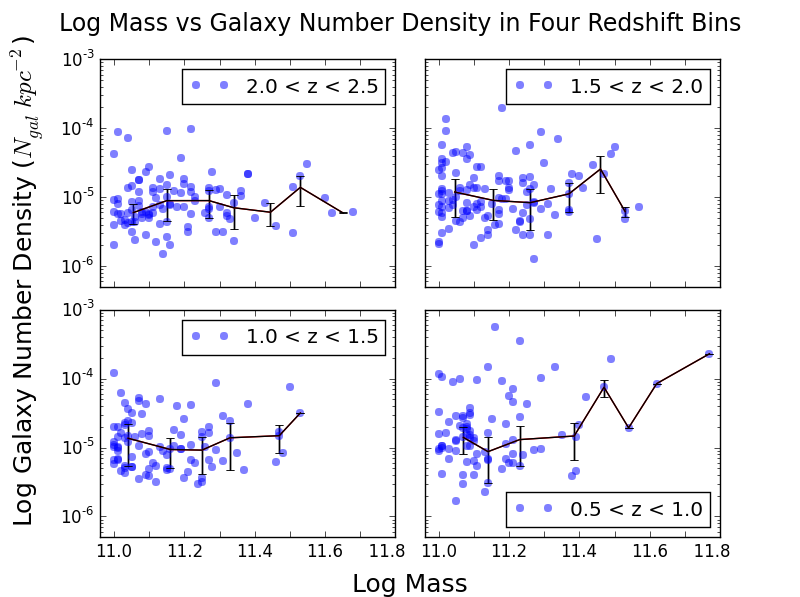
\includegraphics[width=\linewidth]{Mass_Density_Z}
\DeclareGraphicsExtensions{.png}
\caption{\footnotesize All of the galaxies sorted into four bins based on redshift and plotted with mass versus local galaxy number density (both on logarithmic scales). The black line represents the median point of eight mass bins for each subplot. There are error bars for the median absolute deviation of each median point. There is less variation of galaxy density with higher redshifts. An \textbf{\textit{n}} of 5 is used for the nth nearest calculation.}
\label{fig:nth}
\end{figure}

We also plot the data using the nth nearest method in figure~\ref{fig:nth}. In this plot we can analyze change in number density over both redshift and mass. The black line represents the median point for the galaxies, with error bars for the median absolute deviation. The trend of increased galaxy number density with lower redshifts is hard to see, but definively present. One can also notice a general upward trend of galaxy number density with increased mass, as seen in figure~\ref{fig:mass}. Beyond that, one can also see that there is less variation in galaxy number densities for all masses for higher redshifts (smaller error bars).

\begin{figure}
\figurenum{7}
\centering
\graphicspath{{C:/3d_hst/2015_finals/aperture_distance/}}
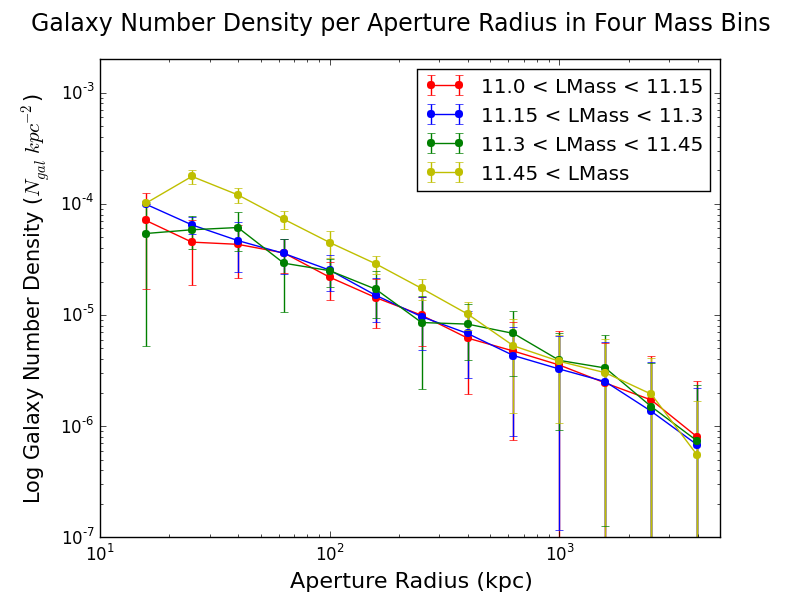
\includegraphics[width=\linewidth]{temp_lmass_final}
\DeclareGraphicsExtensions{.png}
\caption{\footnotesize All of the galaxies sorted into four bins based on mass. Galaxy number density is plotted against selected aperture radius. The error bars represent one standard deviation of the subtracted number density of the randomly selected background points. There is a significant increase in local galaxy number density for extremely high mass galaxies at distances less than 1 one megaparsec.}
\label{fig:mass}
\end{figure}

\subsection{Variation over Satellite Mass}

We also look at the variation in galaxy number density in local and general environments based on the mass of the satellite galaxies. We do this by splitting up all the satellite galaxies into four mass bins: 10 \textsuperscript{9.415}$M_{\odot}$ \textless mass \textless 10 \textsuperscript{9.8}$M_{\odot}$, 10 \textsuperscript{9.8}$M_{\odot}$ \textless mass \textless 10 \textsuperscript{10.3}$M_{\odot}$, 10 \textsuperscript{10.3}$M_{\odot}$ \textless mass \textless 10 \textsuperscript{10.8}$M_{\odot}$, and mass \textgreater 10 \textsuperscript{10.8}$M_{\odot}$. In figure ~\ref{fig:mass_sat} we can see these four bins plotted on an aperture radius graph. The plot shows that in the local environment, there is a greater number density of more massive satellites and a lower number density of less massive satellites. This trend, however, flips in the more general environment (~100kpc and above).

\begin{figure}
\figurenum{8}
\centering
\graphicspath{{C:/3d_hst/2015_finals/aperture_distance/}}
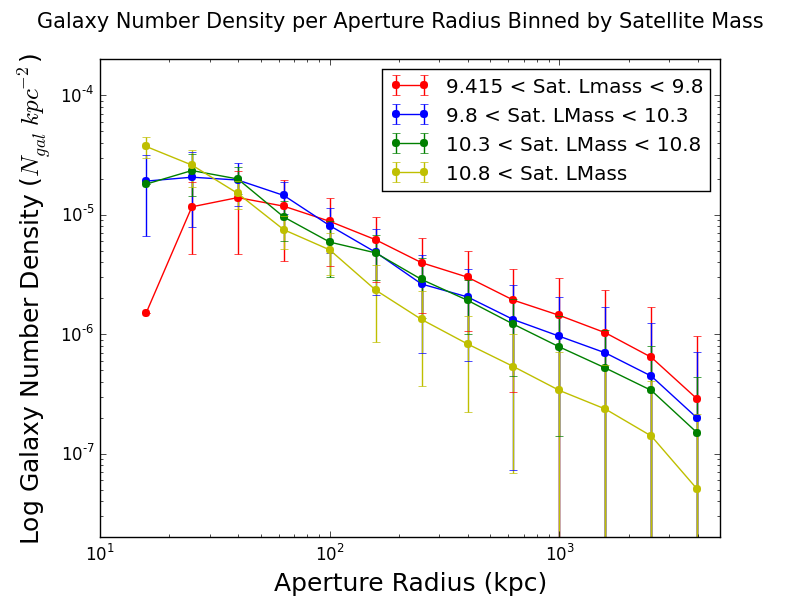
\includegraphics[width=\linewidth]{temp_lmasspanel_final}
\DeclareGraphicsExtensions{.png}
\caption{\footnotesize All galaxies plotted on a galaxy number density versus aperture radius plot split up into four mass bins based on satellite galaxies. In the local environment, there is an increase in number density of more massive satellites. In the general environment, though, there is an icnrease in number density of less massive galaxies.}
\label{fig:mass_sat}
\end{figure}

\subsection{Galaxy Conformity}

Using the star-formation data, we look at galaxy conformity. In figure ~\ref{fig:color_panel} we look at the number density of star-forming and quiescent satellites in the local and general environments of both star-forming and quiescent central galaxies. For star-forming central galaxies, the majority of satellites at all aperture radii are also star-forming. For quiescent centrals, though, there is a majority of quiescent satellites at small aperture radii. The switch to majority star-forming satellites at large aperture radii can be largely explained through the overwhelming majority of star-forming satellites in the total potential satellite sample selection. At large enough aperture radii, the satellites will be dominated by the natural statistical trends of the sample selection. 

It should be noted that the extreme error bars for the quiescent satellites of the star-forming central galaxies is due to the points being an average of so few actual galaxies and creating an extremely large standard deviation. 

In figure ~\ref{fig:conformity1} we calculate the quiescent satellite percentage (F$_{q}$) for all of the central galaxies binned by redshift and star formation color. F$_{q}$ is simply the number of quiescent satellites divided by the total number of satellites within the specified aperture radius. The Quiescent centrals clearly have greater F$_{q}$s for all redshifts, with an increased difference for lower redshifts.

In figure ~\ref{fig:conformity2} we calculate Conformity of each central galaxy bin per aperture radius. The Conformity calculation is simply

$$Conformity = \frac{F_{q} of quiescent centrals - F_{q} of star forming centrals}{F_{q} of all centrals}$$.

There is increased conformity for lower redshifts, with conformity in general going to 0 at high aperture radii.



\begin{figure}
\figurenum{9}
\centering
\graphicspath{{C:/3d_hst/2015_finals/Colors/}}
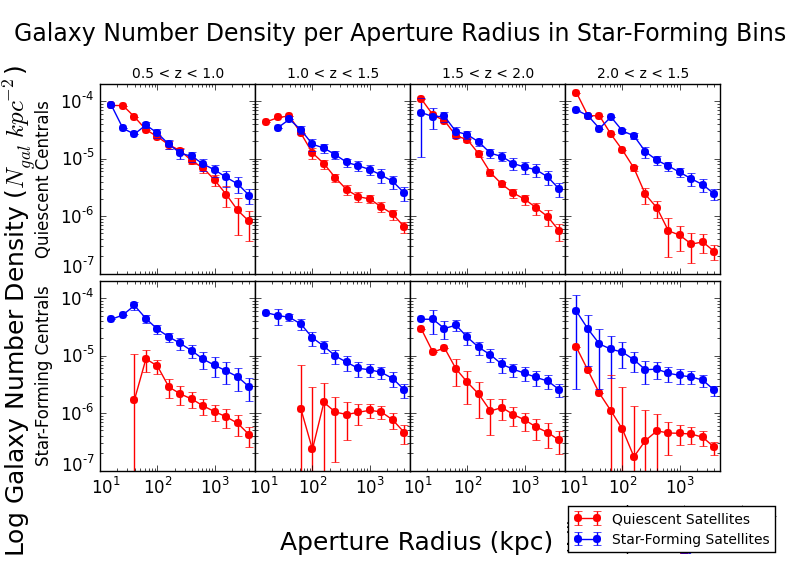
\includegraphics[width=\linewidth]{colorpanel}
\DeclareGraphicsExtensions{.png}
\caption{\footnotesize All of the galaxies sorted into quiescent and star-forming groups plotted separately on an aperture radius versus galaxy number density graph. The satellites of each central galaxy are also sorted in quiescent and star-forming groups, and put on the same sub-plot. There is a correlation between central galaxy type and number density of satellite type at the local environment (small aperture radii). The trned of greater number density of star-formign satellites in the general environment (high aperture radii) can be largely explained through the satellite sample selection.}
\label{fig:color_panel}
\end{figure}

\begin{figure}
\figurenum{10}
\centering
\graphicspath{{C:/3d_hst/2015_finals/Colors/}}
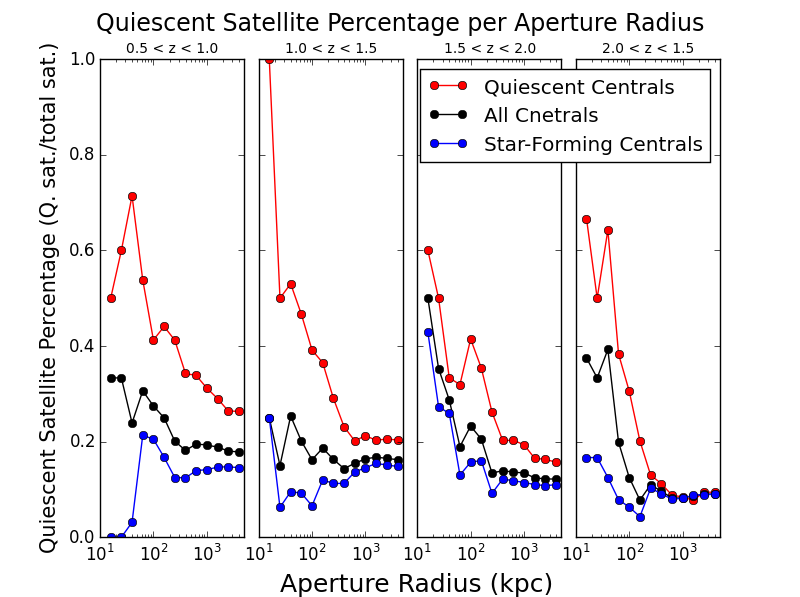
\includegraphics[width=\linewidth]{temp_color_conformity}
\DeclareGraphicsExtensions{.png}
\caption{\footnotesize All central galaxies binned by redshift and star formation color plotted with Quiescent satellite percentage per aperture radius. There is a much greater quiescent satellite percentage for quiescent centrals at all redshifts. However, this difference is smaller for higher redshifts.}
\label{fig:conformity1}
\end{figure}

\begin{figure}
\figurenum{11}
\centering
\graphicspath{{C:/3d_hst/2015_finals/Colors/}}
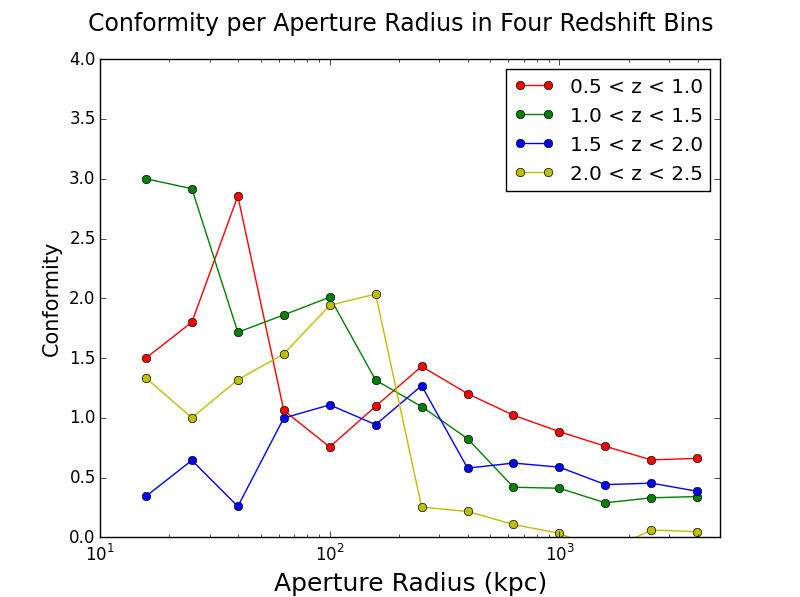
\includegraphics[width=\linewidth]{conformity}
\DeclareGraphicsExtensions{.png}
\caption{\footnotesize All central galaxies binned by redshift plotted with Conformity per aperture radius. Lower redshifts generally have greater conformity.}
\label{fig:conformity2}
\end{figure}

\section{Discussion}

Make some references to how these trends apply to vareious theories? talk about how this compares to results from Kawinwanichakij(2014)~\cite{2014ApJ...792..103K} and Tal(2013)~\cite{2013ApJ...769...31T}.


\acknowledgements

\appendix

\bibliographystyle{plain}
\bibliography{bibliography}

\end{document}
